<<<<<<< HEAD
\begin{name}
	{\tenchude}
	{TOÁN 10}
	{LỚP TOÁN THẦY PHÁT}
	{{Không biết thì không có gì xấu hổ.\\ Chỉ nên cảm thấy xấu hổ khi không chịu học hỏi.}}
\end{name}
\Opensolutionfile{ansbook}[ans/ansbookDe7]
\TN
\Opensolutionfile{ans}[ans/ansDe1-TN7]
\begin{ex}%[0D8N1-5]
Từ các số $1,2,3,4,5,6$ lập được bao nhiêu số tự nhiên gồm $4$ chữ số đôi một khác nhau?
\choice
{\True $360$}
{$15$}
{$1296$}
{$720$}
\loigiai{
Gọi số cần tìm có dạng $\overline{abcd}$.\\
Chọn $a$ có $6$ cách chọn.\\
Chọn $b$ có $5$ cách chọn.\\
Chọn $c$ có $4$ cách chọn.\\
Chọn $d$ có $3$ cách chọn.\\
Theo quy tắc nhân ta có $6 \cdot 5 \cdot 4 \cdot 3=360$ (số).
}
\end{ex}

\begin{ex}%[0D8N2-2]%[HKII-NGUYỄN THÁI BÌNH 2324]%[TheHung Nguyen]
Cho tập $M$ có $12$ phần tử. Số tập con gồm $3$ phần tử của $M$ là
\choice
{$1320$}
{$1728$}
{\True $220$}
{$36$}
\loigiai{
Số tập con gồm $3$ phần tử của $M$ là $\mathrm{C}_{12}^3=220$.
}
\end{ex}

\begin{ex}%[0D8N3-2]
Tìm hệ số của $x^2$  trong khai triển biểu thức $(7x + 5)^{3}$
\choice
{$343$}
{$525$}
{\True $735$}
{$125$}
\loigiai{
Ta viết khai triển biểu thức như sau
\begin{eqnarray*}
(7x + 5)^{3} &=& \mathrm{C}_3^0(7x)^3 + \mathrm{C}_3^1(7x)^25^1 + \mathrm{C}_3^2(7x)^15^2 + \mathrm{C}_3^3(7x)^05^3\\
&=& 343x^3 + 735x^2 + 525x + 125.
\end{eqnarray*}
Suy ra hệ số của $x^2$  trong khai triển là $735$.
}
\end{ex}

\begin{ex}%[H]%[Nguyễn Văn Cường (Cường NV) - Dự án giảng K10 - K11]%[0D6H1-1]
Cho giá trị gần đúng của $\dfrac{23}{7}$ là $3{,}28$. Sai số tuyệt đối của số $3{,}28$ là
\choice
{$0{,}04$}
{\True $\dfrac{0,04}{7}$}
{$0{,}06$}
{Đáp án khác}
\loigiai{
Ta có $\dfrac{23}{7} = 3{,}(285714) \Rightarrow\left|\dfrac{23}{7} - 3{,}28\right| = 0{,}00(571428) = \dfrac{0{,}04}{7}$.}
\end{ex}

\begin{ex}%[0-HK1-CTST-2-NguyenDu-2324]%[VN-MT-6, Lê Minh Thiện Anh]%[0D6H4-2]
Thu thập thông tin về thời gian (giờ) tham gia hoạt động ngoại khóa trong một tháng của học sinh của lớp 10A được cho bởi bảng sau:
\begin{center}
\begin{tabular}{|c|c|c|c|c|c|}
\hline Thời gian (giờ) & $2$ & $3$ & $4$ & $5$ & $6$ \\
\hline Số học sinh lớp 10A & $7$ & $9$ & $10$ & $8$ & $15$ \\
\hline
\end{tabular}
\end{center}
Khoảng biến thiên của lớp 10A là
\choice
{$1$}
{\True $4$}
{$22$}
{$8$}
\loigiai{
Khoảng biến thiên của lớp $10A$ là $R=6-2=4$.
}
\end{ex}

\begin{ex}%[0D0N1-2]%[Dự án đề kiểm tra Toán khối 10 HKI NH23-24-Dot 15- Hồ Văn Trung]%[THPT Lê Qúy Đôn- TPHCM]
Bạn Minh muốn nuôi một trong bốn con vật sau: mèo, chó, chim, cá. Bạn Minh đã chọn ngẫu nhiên một con vật. Tập hợp nào sau đây \textbf{không phải} là một biến cố của phép thử trên?
\choice
{$H=\varnothing $}
{$K= \{ \text{mèo, chó, chim, cá}\}$}
{\True $J= \{ \text{mèo, chim, thỏ}\}$}
{$I= \{ \text{chó, cá}\}$}
\loigiai{Ta có thỏ không phải là con vật bạn Minh nuôi.\\
Nên tập $J= \{ \text{mèo, chim, thỏ}\}$ không phải là một biến cố của phép thử trên.
}
\end{ex}

\begin{ex}%[0D0N1-3]
Một cửa hàng có $23$ chiếc kem que khác nhau và $7$ chiếc kem ốc quế khác nhau. Chọn ngẫu nhiên một chiếc kem que và một chiếc kem ốc quế. Số phần tử của không gian mẫu là
\choice
{\True $161$}
{$30$}
{$35$}
{$435$}
\loigiai{
Số phần tử của không gian mẫu là $n(\Omega)=23\cdot7=161$.
}
\end{ex}

\begin{ex}%[10-11-EX-GHK2-2425]%[Lê Toàn]%[0H9H3-1]
Cho đường thẳng $d \colon \heva{&x=5+t \\&y=-9-2t}$; khẳng định nào sau đây \textbf{sai}?
\choice
{$d$ có véc-tơ chỉ phương $(1;-2)$}
{$d$ có véc-tơ pháp tuyến $(2;1)$}
{$d$ có véc-tơ chỉ phương $(2;-4)$}
{\True $d$ có véc-tơ pháp tuyến $(2;-1)$}
\loigiai{
Đường thẳng $d$ có véc-tơ chỉ phương $\overrightarrow{u}=(1;-2)$  nên có một véc-tơ pháp tuyến là $\overrightarrow{n}=(2;1)$.
}
\end{ex}

\begin{ex}%[0H9H3-2]%[Dự án đề kiểm tra Toán 11 GHKII NH23-24-Nguyen Tran Anh Tuan]%[THPT Thiệu Hóa - Thanh Hóa]
Trong mặt phẳng tọa độ $Oxy$ đường thẳng đi qua $A(-1; 4)$ và song song trục $Ox$ có phương trình là
\choice
{$x-1=0$}
{$y+4=0$}
{$x+1=0$}
{\True $y-4=0$}
\loigiai{
Gọi $d$ là đường thẳng cần tìm.\\
Vì $d \parallel Ox \Rightarrow \overrightarrow{u_d}=\overrightarrow{u}_{Ox}=(1; 0)$ suy ra $\overrightarrow{n_d}=(0;-1)$.\\
Phương trình tổng quát của $d$ là $(d)\colon 0(x+1)-1(y-4)=0$ hay $ y-4=0$.
}
\end{ex}

\begin{ex}%[0H9H3-4]%[Tex hóa đề CK2 - form 2025 - đọt 2 -Huỳnh Thanh Chí]
Cho 2 đường thẳng $\Delta\colon x-y+2=0$ và $\Delta'\colon-x+1=0$. Góc giữa 2 đường thẳng $\Delta$ và $\Delta'$ bằng
\choice
{$90^{\circ}$}
{$135^{\circ}$}
{\True $45^\circ$}
{$60^{\circ}$}
\loigiai{Ta có véc-tơ pháp tuyến của $\Delta$ là $\overrightarrow{n}=(1;-1)$, véc-tơ pháp tuyến $\Delta'$ là $\overrightarrow{n}'=(1; 0)$.\\
Ta có $
\cos \left(\Delta, \Delta'\right)=\left|\cos \left(\overrightarrow{n}, \overrightarrow{n}'\right)\right|=\dfrac{\sqrt{2}}{2} \Rightarrow\left(\Delta, \Delta'\right)=45^{\circ}$.
}
\end{ex}

\begin{ex}%[0H9N5-1]
Trong mặt phẳng $O x y$, tọa độ các tiêu điểm của elip có phương trình chính tắc \break $\dfrac{x^2}{25}+\dfrac{y^2}{16}=1$ là
\choice
{\True $F_1(-3 ; 0)$; $F_2(3 ; 0)$}
{$F_1(0 ;-4)$; $F_2(0 ; 4)$}
{$F_1(-4 ; 0)$; $F_2(4 ; 0)$}
{$F_1(0 ;-3)$; $F_2(0 ; 3)$}
\loigiai{ Ta có $\heva{&a^2=25\\&b^2=16}\Rightarrow c^2=a^2-b^2=25-16=9.$\\
Tọa độ các tiêu điểm của elip là $F_1(-3 ; 0)$; $F_2(3 ; 0)$.
}
\end{ex}

\begin{ex}%[0H9N5-5]%[Dự án đề kiểm tra Toán 10 HKII NH23-24- Đoàn Minh Tâm]%[THPT Mạc Đĩnh Chi]
Trong mặt phẳng tọa độ $Oxy$, hypebol $(H)$ có độ dài trục thực bằng $ 6$ và tiêu cự bằng $ 10$ có phương trình chính tắc là
\choice
{\True $(H)\colon\dfrac{x^2}{9}-\dfrac{y^2}{16}=1$}
{$(H)\colon\dfrac{x^2}{16}-\dfrac{y^2}{9}=1$}
{$(H)\colon\dfrac{x^2}{25}-\dfrac{y^2}{9}=1$}
{$(H)\colon\dfrac{x^2}{36}-\dfrac{y^2}{64}=1$}
\loigiai{
Độ dài trục thực bằng $6$ nên $2a=6 \Rightarrow a=3\Rightarrow a^2=9$.\\
Tiêu cự bằng $10$ nên $2c=10 \Rightarrow c=5$.\\
Ta có $b^2=c^2-a^2=25-9=16$.\\
Vậy phương trình chính tắc của hypebol $(H)$ là $\dfrac{x^2}{9}-\dfrac{y^2}{16}=1$.
}
\end{ex}
\TNTF
\begin{ex}%[Chuẩn hóa M25, Nguyễn Văn Nay]%[0D8V2-5]
Từ một hộp chứa $30$ quả cầu được đánh số từ $1$ đến $30$, chọn ngẫu nhiên $4$ quả cầu.
\choiceTF[t]
{\True Có $27\,405$ cách chọn}
{Có $1\,365$ cách chọn để tích các số trên các quả cầu là số chẵn}
{\True Có $13\,755$ cách chọn để tổng số trên các quả cầu là số chẵn}
{\True Có $13\,755$ cách chọn để tổng bình phương các số trên các quả cầu là số chẵn}
\loigiai{
\begin{itemchoice}
\itemch Số cách chọn ngẫu nhiên $4$ quả cầu là $\mathrm{C}_{30}^4=27\,405$ cách.
\itemch Để tích các số trên quả cầu là số chẵn thì ít nhất một số là số chẵn.\\
Số cách chọn $4$ số đều lẻ là $\mathrm{C}_{15}^4$.\\
Suy ra số cách chọn để có ít nhất một số chẵn là $\mathrm{C}_{30}^4-\mathrm{C}_{15}^4=26\,040$ cách.
\itemch Để tổng số trên các quả cầu là số chẵn, ta có các trường hợp
\begin{itemize}
\item \textbf{TH1.} Chọn $4$ số chẵn trong các số từ $1$ đến $30$ có $\mathrm{C}_{15}^4$.
\item \textbf{TH2.} Chọn $2$ số chẵn và $2$ số lẻ trong các số từ $1$ đến $30$ có $\mathrm{C}_{15}^2\cdot\mathrm{C}_{15}^2$.
\item \textbf{TH3.} Chọn $4$ số lẻ trong các số từ $1$ đến $30$ có $\mathrm{C}_{15}^4$.
\end{itemize}
Vậy có $2 \cdot \mathrm{C}_{15}^4 +\mathrm{C}_{15}^2\cdot\mathrm{C}_{15}^2=13\,755$ (cách chọn)
\itemch Vì bình phương của một số không làm thay đổi tính chẵn, lẻ, nên để tổng bình phương các số là số chẵn thì tổng các số là số chẵn.\\
Theo ý b), ta có $13\,755$ cách.
\end{itemchoice}
}
\end{ex}

\begin{ex}%[0H9H3-2]%[Làm đề GHK, HK, 4 phần - 2025]%[Huỳnh Xuân Tín]
Trong mặt phẳng toạ độ $Oxy$, cho tam giác $ABC$ có $A(3; 4)$, đường trung trực cạnh $BC$ có phương trình $3x-y+1=0$, đường trung tuyến kẻ từ $C$ có phương trình $2x-y+5=0$. Xét tính đúng sai các mệnh đề sau
\choiceTF
{Gọi $M$ là trung điểm cạnh $BC$. Khi đó $M(9; 39)$}
{\True Phương trình đường thẳng $BC$ là $x+3y-63=0$}
{Tọa độ đỉnh $C$ là $C(-1; 3)$}
{\True Tọa độ đỉnh $B$ là $B\left(\dfrac{15}{7}; \dfrac{142}{7}\right)$}
\loigiai{
\begin{itemchoice}
\itemch Sai. Gọi $M$ là trung điểm cạnh $BC$. Vì $M$ nằm trên đường trung trực cạnh $BC$ nên giả sử $M\ (t; 3t+1)$.\\
Gọi $G$ là trọng tâm tam giác $ABC$. Vì $G$ nằm trên đường trung tuyền kẻ từ $C$ nên giả sử $G\ (s; 2s+5)$.\\
Ta có $\heva{& \overrightarrow{A M}=(t-3; 3 t-3)\\&\overrightarrow{A G}=(s-3; 2 s+1).}$\\
Khi đó
\begin{eqnarray*}
& &\overrightarrow{A M}=\dfrac{3}{2} \overrightarrow{A G}\\ &\Leftrightarrow&\heva{&t-3=\dfrac{3}{2}(s-3)\\&3t-3=\dfrac{3}{2}(2s+1)}\\
&\Leftrightarrow& \heva{&{2t-3s=-3} \\&{6t-6s=9}}\\
&\Leftrightarrow& \heva{&t=\dfrac{15}{2} \\	&s=6.}
\end{eqnarray*}
Suy ra $M\left(\dfrac{9}{2}; \dfrac{39}{2}\right)$.
\itemch Đúng. Đường thẳng $BC$ đi qua $M\left(\dfrac{9}{2}; \dfrac{39}{2}\right)$ và vuông góc với đường thẳng $3x-y+1=0$ nên ta có phương trình đường thẳng $BC$ là\\ $1\cdot\left(x-\dfrac{9}{2}\right)+3\cdot\left(y-\dfrac{39}{2}\right)=0\Leftrightarrow x+3y-63=0$.
\itemch Sai. Toạ độ đỉnh $C$ là nghiệm của hệ phương trình $\heva{&x+3y-63=0\\
&2x-y+5=0} \Leftrightarrow\heva{&x=\dfrac{48}{7} \\&y=\dfrac{131}{7}.}$
\itemch Đúng. Ta có $C\left(\dfrac{48}{7}; \dfrac{131}{7}\right)$.Vì $M$ là trung điểm $BC$ nên $B\left(\dfrac{15}{7}; \dfrac{142}{7}\right)$.
\end{itemchoice}}
\end{ex}
\TNSA
\begin{ex}%[10-11-12EX-GK2-2425]%[Trần Văn Hùng]%[0D8V1-2]
Bạn Sơn muốn bố trí một hệ thống $12$ bóng đèn màu trên chiếc cửa sổ phòng học của mình. Theo tư vấn của một người bạn, Sơn quyết định chọn $3$ màu khác nhau cho số bóng đèn này với điều kiện $2$ bóng đèn kề nhau (được nối với nhau bằng $1$ đoạn dây như hình) thì không có cùng màu. Hỏi Sơn có bao nhiêu cách chọn màu cho $12$ bóng đèn như thế?
\begin{center}
\begin{tikzpicture}[scale=0.4, font=\footnotesize, line join=round, line cap=round, >=stealth]
%Vẽ đường tròn
\foreach \x/\y in {-11/0,-7/0, -3/0, 3/0, 7/0,11/0, 0/3, 0/7,0/11, 0/-3, 0/-7,0/-11}
\node[circle, draw, minimum size=0.8cm] at (\x,\y) {};
\draw (-10,0)--(-8,0) (-6,0)--(-4,0) (0,4)--(0,6) (0,8)--(0,10)
(0,-10)--(0,-8) (0,-6)--(0,-4) (4,0)--(6,0) (8,0)--(10,0)
(2.2,0.6)--(0.7,2.3) (-2.2,0.6)--(-0.7,2.3)
(-0.7,-2.3)--(-2.2,-0.6) (0.7,-2.3)--(2.2,-0.6)
;
\end{tikzpicture}
\end{center}
\loigiai
{
\immini[thm]{
Đánh số thứ tự các quả bóng như hình vẽ.\\
Chọn màu cho quả bóng số $1$, có $3$ cách chọn.\\
Chọn màu cho quả bóng số $2$, có $2$ cách chọn.\\
Chọn màu cho quả bóng số $3$, có $2$ cách chọn.\\
Chọn màu cho quả bóng số $9$, có $2$ cách chọn.\\
Chọn màu cho quả bóng số $8$, có $2$ cách chọn.\\
Chọn màu cho quả bóng số $7$, có $2$ cách chọn.\\
Chọn màu cho quả bóng số $4$, có $2$ cách chọn.\\
Chọn màu cho quả bóng số $5$, có $2$ cách chọn.\\
Chọn màu cho quả bóng số $6$, có $2$ cách chọn.\\
Chọn màu cho quả bóng số $10$, có $1$ cách chọn.\\
Chọn màu cho quả bóng số $11$, có $2$ cách chọn.\\
Chọn màu cho quả bóng số $12$, có $2$ cách chọn.\\
Vậy có $3\cdot 2^{10}\cdot 1=3072$ cách.
}
{




\begin{tikzpicture}[scale=0.4, font=\footnotesize, line join=round, line cap=round, >=stealth]
%Vẽ đường tròn
\foreach \x/\y in {-11/0,-7/0, -3/0, 3/0, 7/0,11/0, 0/3, 0/7,0/11, 0/-3, 0/-7,0/-11}
\node[circle, draw, minimum size=0.8cm] at (\x,\y) {};
\draw (-10,0)--(-8,0) (-6,0)--(-4,0) (0,4)--(0,6) (0,8)--(0,10)
(0,-10)--(0,-8) (0,-6)--(0,-4) (4,0)--(6,0) (8,0)--(10,0)
(2.2,0.6)--(0.7,2.3) (-2.2,0.6)--(-0.7,2.3)
(-0.7,-2.3)--(-2.2,-0.6) (0.7,-2.3)--(2.2,-0.6)
;
\draw (-11,0)node[]{$1$} (-7,0)node[]{$2$} (-3,0)node[]{$3$}
(3,0)node[]{$4$} (7,0)node[]{$5$} (11,0)node[]{$6$}
(0,3)node[]{$9$} (0,7)node[]{$8$} (0,11)node[]{$7$}
(0,-3)node[]{$10$} (0,-7)node[]{$11$} (0,-11)node[]{$12$}
;
\end{tikzpicture}
}

}
\end{ex}

\begin{ex}%[HSA-đợt 1-Trần Như Cang]%[0D8V3-4]
Hệ số của $x^{10}$ trong khai triển $\left(1+x+x^2+x^3\right)^5$ bằng bao nhiêu?
\shortans{101}
\loigiai{
Theo khai triển nhị thức Newton, ta có
\[\left(1+x+x^2+x^3\right)^5=(1+x)^5\left(1+x^2\right)^5=\sum _{k=0}^5\mathrm{C}_5^k x^k\cdot \sum _{l=0}^5\mathrm{C}_5^l (x^2)^l=\sum _{k=0}^5\mathrm{C}_5^k\cdot\sum _{l=0}^5\mathrm{C}_5^l\cdot x^{k+2l}.
\]
Số hạng chứa $x^{10}$ trong khai triển tương ứng với $k+2l=10\Leftrightarrow k=10-2l$.\\
Kết hợp với điều kiện ta có hệ $\heva{&k+2l=10\\&0\le k\le 5,\,0\le l\le5\\&k,l\in\mathbb{N}}\Leftrightarrow(k;l)=\left\lbrace  (0;5),(2;4),(4;3)\right\rbrace $.\\
Vậy hệ số cần tìm là $\mathrm{C}_5^0\cdot \mathrm{C}_5^5+\mathrm{C}_5^2\cdot \mathrm{C}_5^4+\mathrm{C}_5^4\cdot \mathrm{C}_5^3=101$.
}
\end{ex}

\begin{ex}%[0-HK1-CT-4-THTHDHSG-HCM-2324]%[VN-MT-6, VM026]%[0D6H3-2]
Thống kê độ tuổi kiếm được việc làm đúng chuyên ngành sau khi tốt nghiệp đại học của một nhóm người, thu được bảng sau
\begin{center}
\begin{tabular}{|c|c|c|c|c|c|}
\hline
Tuổi		& 22& 23& 24& 25& 26 \\
\hline
Số người 	& 12& 20& 19& 8& 5\\
\hline
\end{tabular}
\end{center}
Tính độ tuổi trung bình của nhóm người này khi họ kiếm được việc làm đúng chuyên ngành (kết quả làm tròn đến chữ số hàng phần mười).
\shortans{$23{,}6$}
\loigiai{
Ta có, cỡ mẫu $n=12+20+19+8+5=64$.\\
Độ tuổi trung bình của nhóm người này khi họ kiếm được việc làm đúng chuyên ngành được tính là
\[\overline{x}=\dfrac{12\cdot 22 + 20 \cdot 23 + 19 \cdot 24 + 8 \cdot 25+5 \cdot 26}{64}=\dfrac{1510}{64}\approx23{,}6.\]
}
\end{ex}

\begin{ex}%[0H9V4-2]
Trong mặt phẳng với hệ tọa độ $Oxy$, cho đường thẳng $d\colon 2x-y-5=0$ và hai điểm $A\left(1;2\right), B\left(4;1\right)$. Tính bán kính đường tròn $(C)$ có tâm thuộc $d$ và đi qua hai điểm $A, B$.
\shortans{$5$}
\loigiai{
\immini[thm]{
Gọi $I$ là tâm của $(C)$. Do $I\in d$ nên $I\left(t;2t-5\right)$.\\
Hai điểm $A, B$ cùng thuộc $(C)$ nên
\begin{align*}
IA=IB & \Leftrightarrow (1-t)^2+\left(7-2t\right)^2=(4-t)^2+\left(6-2t\right)^2\\
& \Leftrightarrow t=1.
\end{align*}
Suy ra $I(1;-3)$ và bán kính $R=IA=5$.\\

}
{
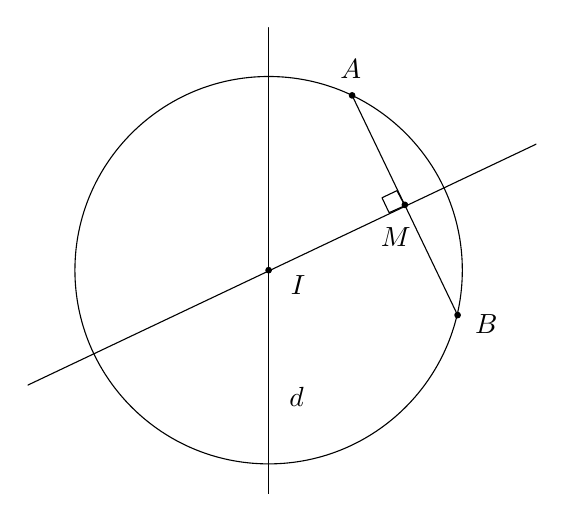
\begin{tikzpicture}[line cap=round,line join=round,>=stealth,x=1.0cm,y=1.0cm]
\clip(1.24,-1.) rectangle (7.7,4.92);
\draw (5.93,2.85) -- (5.74,2.76) -- (5.83,2.57) -- (6.03,2.66) -- cycle;
\draw (4.3,1.84) circle (2.46cm);
\draw (5.36,4.06)-- (6.7,1.27);
\draw [domain=1.24:7.7] plot(\x,{(-0.36--0.82*\x)/1.73});
\draw (4.3,-1.) -- (4.3,4.92);
\draw (5.6,4.4) node[left] {$A$};
\draw (6.8,1.4) node[anchor=north west] {$B$};
\draw (5.6,2.5) node[anchor=north west] {$M$};
\draw (4.44,0.48) node[anchor=north west] {$d$};
\draw (4.46,1.9) node[anchor=north west] {$I$};
\draw [fill=black] (4.3,1.84) circle (1.0pt);
\draw [fill=black] (5.36,4.06) circle (1.0pt);
\draw [fill=black] (6.7,1.27) circle (1.0pt);
\draw [fill=black] (6.03,2.67) circle (1.0pt);
\end{tikzpicture}
}
}
\end{ex}
\TL
\begin{ex}%[0H9H3-2]%[Dự án đề kiểm tra Toán 10 HKII NH23-24-Đỗ Chí Tâm]%[THPT Đặng Huy Trứ- Huế]
Trong mặt phẳng với hệ trục tọa độ $Oxy$, cho hai điểm $A(2;-3), B(4;1)$. Gọi $\Delta$ là đường thẳng trung trực của đoạn $AB$. Viết phương trình tham số của đường thẳng $\Delta$.
\loigiai{
Trung điểm của $AB$ là $I(3;-1)$.\\
Vectơ pháp tuyến của đường thẳng $\Delta$ là $\vec{n_{\Delta}}=\vec{AB}=(2;4)$.\\
Đường thẳng $\Delta$ đi qua trung điểm $I(3;-1)$ của $AB$ và có vectơ chỉ phương $\vec{u_{\Delta}}=(4;-2)$, có phương trình là $\heva{&x=3+4t\\&y=-1-2t}\quad t\in\mathbb{R}$.

}
\end{ex}

\begin{ex}%[0H9V4-5]%[Dự án đề kiểm tra Toán 10 HKII NH23-24- Trung Anh]%[THPT Việt Đức - Hà Nội]
Trong mặt phẳng với hệ trục tọa độ $Oxy$, cho đường tròn $(C): x^2+y^2+4x-2y-20=0$ và đường thẳng $\triangle: 3x+4y-m=0$. Tìm giá trị dương của tham số $m$ để đường thẳng $\triangle$ cắt đường tròn $(C)$ theo một dây dung có độ dài bằng $6$.
\loigiai{
\begin{center}
\begin{tikzpicture}[declare function={r=2.5;ga=40;},>=stealth,font=\scriptsize,scale=0.8]
%\path (0:0) coordinate (I)
%(ga:r) coordinate (A)
%(130:r) coordinate (B)
\coordinate (I) at (0,0);
\coordinate (A) at (ga:r);
\coordinate (B) at (130:r);
\coordinate (J) at ($(A)!1/2!(B)$);
\draw (I) circle (r)  ;
\draw (I)--(A)--(B)--(I)--(J);
\foreach \x/\g in{A/90,B/90,J/90,I/-90}
\fill[black](\x) circle (2pt)
($(\x)+(\g:5mm)$) node{\small $\x$};
\end{tikzpicture}
\end{center}
Đường tròn $(C)$ có tâm $I(-2;1)$ và bán kính $R=\sqrt{(-2)^2+1^2+20}=5$.\\
Giả sử $\triangle$ cắt $(C)$ tại hai điểm $A$ và $B$. Gọi $J$ là trung điểm của $AB$.\\
Khi đó $\heva{&IJ\perp AB\\&JB=\dfrac{1}{2}AB=3.}$\\
Xét tam giác $IJB$ vuông tại $J$ có \[IJ=\sqrt{IB^2-JB^2}=4.\]
Hay $\mathrm{d}(I; \triangle)=4$. Tương đương
\begin{align*}
&\dfrac{|(-2)\cdot3+4\cdot1-m|}{\sqrt{3^+4^2}}=4\\
\Leftrightarrow&\, |m+2|=4\cdot5=20\\
\Leftrightarrow&\, \hoac{&m+2=20\\&m+2=-20}\Leftrightarrow\hoac{&m=18\\&m=-22\,(\text{không thỏa mãn}).}
\end{align*}
Vậy $m=18$.
}
\end{ex}

\begin{ex}%[Phan Quốc Trí]%[0D0C2-7]
Gọi $X$ là tập hợp các số tự nhiên chẵn có $4$ chữ số khác nhau được lập từ các chữ	số $0$; $2$; $3$; $4$; $5$; $6$; $7$. Chọn ngẫu nhiên một số thuộc tập $X$. Tính xác suất để số được chọn chia hết cho $4$ (làm tròn đến hàng phần nghìn).
% \shortans{$0{,}495$}
\loigiai
{
Gọi $\overline{abcd}$ là số tự nhiên chẵn có $4$ chữ số khác nhau được lập từ các chữ số $0$; $2$; $3$; $4$; $5$; $6$; $7$.\\ Các khả năng xảy ra là
\begin{itemize}
\item $d=0$: $a$ có $6$ cách chọn, $b$ có $5$ cách chọn, $c$ có $4$ cách chọn. Có $6\cdot 5\cdot 4=120$ số như vậy.
\item $d\in \{2;4;6\}\Rightarrow d$ có $3$ cách chọn, $a$ có $5$ cách chọn, $b$ có $5$ cách chọn, $c$ có $4$ cách chọn. Có $3\cdot 5\cdot 5\cdot 4=300$ số như vậy.
\end{itemize}
Số phần tử của không gian mẫu là $n(\Omega)=120+300=420$.\\
Gọi $A$ là biến cố \lq\lq Số được chọn chia hết cho $4$\rq\rq.\\
Các khả năng xảy ra là
\begin{itemize}
\item $\overline{cd}\in \{04;20;40;60\}$, $\overline{cd}$ có $4$ cách chọn, $a$ có $5$ cách chọn, $b$ có $4$ cách chọn. Có $4\cdot 5\cdot 4=80$ số như vậy.
\item $\overline{cd}\in \{24;32;36;52;56;64;72;76\}$, $\overline{cd}$ có $8$ cách chọn, $a$ có $4$ cách chọn, $b$ có $4$ cách chọn.\\ Có $8\cdot 4\cdot 4=128$ số như vậy.
\end{itemize}
Số phần tử của biến cố $A$ là $n(A)=80+128=208$.\\
Xác suất cần tìm là $\mathrm{P}(A)=\dfrac{n(A)}{n(\Omega)}=\dfrac{208}{420}=\dfrac{52}{105} \approx 0{,}495$.
}
\end{ex}
\Closesolutionfile{ans}
\Closesolutionfile{ansbook}
=======
\begin{name}
	{\tenchude}
	{TOÁN 10}
	{LỚP TOÁN THẦY PHÁT}
	{{Không biết thì không có gì xấu hổ.\\ Chỉ nên cảm thấy xấu hổ khi không chịu học hỏi.}}
\end{name}
\Opensolutionfile{ansbook}[ans/ansbookDe7]
\TN
\Opensolutionfile{ans}[ans/ansDe1-TN7]
\begin{ex}%[0D8N1-5]
Từ các số $1,2,3,4,5,6$ lập được bao nhiêu số tự nhiên gồm $4$ chữ số đôi một khác nhau?
\choice
{\True $360$}
{$15$}
{$1296$}
{$720$}
\loigiai{
Gọi số cần tìm có dạng $\overline{abcd}$.\\
Chọn $a$ có $6$ cách chọn.\\
Chọn $b$ có $5$ cách chọn.\\
Chọn $c$ có $4$ cách chọn.\\
Chọn $d$ có $3$ cách chọn.\\
Theo quy tắc nhân ta có $6 \cdot 5 \cdot 4 \cdot 3=360$ (số).
}
\end{ex}

\begin{ex}%[0D8N2-2]%[HKII-NGUYỄN THÁI BÌNH 2324]%[TheHung Nguyen]
Cho tập $M$ có $12$ phần tử. Số tập con gồm $3$ phần tử của $M$ là
\choice
{$1320$}
{$1728$}
{\True $220$}
{$36$}
\loigiai{
Số tập con gồm $3$ phần tử của $M$ là $\mathrm{C}_{12}^3=220$.
}
\end{ex}

\begin{ex}%[0D8N3-2]
Tìm hệ số của $x^2$  trong khai triển biểu thức $(7x + 5)^{3}$
\choice
{$343$}
{$525$}
{\True $735$}
{$125$}
\loigiai{
Ta viết khai triển biểu thức như sau
\begin{eqnarray*}
(7x + 5)^{3} &=& \mathrm{C}_3^0(7x)^3 + \mathrm{C}_3^1(7x)^25^1 + \mathrm{C}_3^2(7x)^15^2 + \mathrm{C}_3^3(7x)^05^3\\
&=& 343x^3 + 735x^2 + 525x + 125.
\end{eqnarray*}
Suy ra hệ số của $x^2$  trong khai triển là $735$.
}
\end{ex}

\begin{ex}%[H]%[Nguyễn Văn Cường (Cường NV) - Dự án giảng K10 - K11]%[0D6H1-1]
Cho giá trị gần đúng của $\dfrac{23}{7}$ là $3{,}28$. Sai số tuyệt đối của số $3{,}28$ là
\choice
{$0{,}04$}
{\True $\dfrac{0,04}{7}$}
{$0{,}06$}
{Đáp án khác}
\loigiai{
Ta có $\dfrac{23}{7} = 3{,}(285714) \Rightarrow\left|\dfrac{23}{7} - 3{,}28\right| = 0{,}00(571428) = \dfrac{0{,}04}{7}$.}
\end{ex}

\begin{ex}%[0-HK1-CTST-2-NguyenDu-2324]%[VN-MT-6, Lê Minh Thiện Anh]%[0D6H4-2]
Thu thập thông tin về thời gian (giờ) tham gia hoạt động ngoại khóa trong một tháng của học sinh của lớp 10A được cho bởi bảng sau:
\begin{center}
\begin{tabular}{|c|c|c|c|c|c|}
\hline Thời gian (giờ) & $2$ & $3$ & $4$ & $5$ & $6$ \\
\hline Số học sinh lớp 10A & $7$ & $9$ & $10$ & $8$ & $15$ \\
\hline
\end{tabular}
\end{center}
Khoảng biến thiên của lớp 10A là
\choice
{$1$}
{\True $4$}
{$22$}
{$8$}
\loigiai{
Khoảng biến thiên của lớp $10A$ là $R=6-2=4$.
}
\end{ex}

\begin{ex}%[0D0N1-2]%[Dự án đề kiểm tra Toán khối 10 HKI NH23-24-Dot 15- Hồ Văn Trung]%[THPT Lê Qúy Đôn- TPHCM]
Bạn Minh muốn nuôi một trong bốn con vật sau: mèo, chó, chim, cá. Bạn Minh đã chọn ngẫu nhiên một con vật. Tập hợp nào sau đây \textbf{không phải} là một biến cố của phép thử trên?
\choice
{$H=\varnothing $}
{$K= \{ \text{mèo, chó, chim, cá}\}$}
{\True $J= \{ \text{mèo, chim, thỏ}\}$}
{$I= \{ \text{chó, cá}\}$}
\loigiai{Ta có thỏ không phải là con vật bạn Minh nuôi.\\
Nên tập $J= \{ \text{mèo, chim, thỏ}\}$ không phải là một biến cố của phép thử trên.
}
\end{ex}

\begin{ex}%[0D0N1-3]
Một cửa hàng có $23$ chiếc kem que khác nhau và $7$ chiếc kem ốc quế khác nhau. Chọn ngẫu nhiên một chiếc kem que và một chiếc kem ốc quế. Số phần tử của không gian mẫu là
\choice
{\True $161$}
{$30$}
{$35$}
{$435$}
\loigiai{
Số phần tử của không gian mẫu là $n(\Omega)=23\cdot7=161$.
}
\end{ex}

\begin{ex}%[10-11-EX-GHK2-2425]%[Lê Toàn]%[0H9H3-1]
Cho đường thẳng $d \colon \heva{&x=5+t \\&y=-9-2t}$; khẳng định nào sau đây \textbf{sai}?
\choice
{$d$ có véc-tơ chỉ phương $(1;-2)$}
{$d$ có véc-tơ pháp tuyến $(2;1)$}
{$d$ có véc-tơ chỉ phương $(2;-4)$}
{\True $d$ có véc-tơ pháp tuyến $(2;-1)$}
\loigiai{
Đường thẳng $d$ có véc-tơ chỉ phương $\overrightarrow{u}=(1;-2)$  nên có một véc-tơ pháp tuyến là $\overrightarrow{n}=(2;1)$.
}
\end{ex}

\begin{ex}%[0H9H3-2]%[Dự án đề kiểm tra Toán 11 GHKII NH23-24-Nguyen Tran Anh Tuan]%[THPT Thiệu Hóa - Thanh Hóa]
Trong mặt phẳng tọa độ $Oxy$ đường thẳng đi qua $A(-1; 4)$ và song song trục $Ox$ có phương trình là
\choice
{$x-1=0$}
{$y+4=0$}
{$x+1=0$}
{\True $y-4=0$}
\loigiai{
Gọi $d$ là đường thẳng cần tìm.\\
Vì $d \parallel Ox \Rightarrow \overrightarrow{u_d}=\overrightarrow{u}_{Ox}=(1; 0)$ suy ra $\overrightarrow{n_d}=(0;-1)$.\\
Phương trình tổng quát của $d$ là $(d)\colon 0(x+1)-1(y-4)=0$ hay $ y-4=0$.
}
\end{ex}

\begin{ex}%[0H9H3-4]%[Tex hóa đề CK2 - form 2025 - đọt 2 -Huỳnh Thanh Chí]
Cho 2 đường thẳng $\Delta\colon x-y+2=0$ và $\Delta'\colon-x+1=0$. Góc giữa 2 đường thẳng $\Delta$ và $\Delta'$ bằng
\choice
{$90^{\circ}$}
{$135^{\circ}$}
{\True $45^\circ$}
{$60^{\circ}$}
\loigiai{Ta có véc-tơ pháp tuyến của $\Delta$ là $\overrightarrow{n}=(1;-1)$, véc-tơ pháp tuyến $\Delta'$ là $\overrightarrow{n}'=(1; 0)$.\\
Ta có $
\cos \left(\Delta, \Delta'\right)=\left|\cos \left(\overrightarrow{n}, \overrightarrow{n}'\right)\right|=\dfrac{\sqrt{2}}{2} \Rightarrow\left(\Delta, \Delta'\right)=45^{\circ}$.
}
\end{ex}

\begin{ex}%[0H9N5-1]
Trong mặt phẳng $O x y$, tọa độ các tiêu điểm của elip có phương trình chính tắc \break $\dfrac{x^2}{25}+\dfrac{y^2}{16}=1$ là
\choice
{\True $F_1(-3 ; 0)$; $F_2(3 ; 0)$}
{$F_1(0 ;-4)$; $F_2(0 ; 4)$}
{$F_1(-4 ; 0)$; $F_2(4 ; 0)$}
{$F_1(0 ;-3)$; $F_2(0 ; 3)$}
\loigiai{ Ta có $\heva{&a^2=25\\&b^2=16}\Rightarrow c^2=a^2-b^2=25-16=9.$\\
Tọa độ các tiêu điểm của elip là $F_1(-3 ; 0)$; $F_2(3 ; 0)$.
}
\end{ex}

\begin{ex}%[0H9N5-5]%[Dự án đề kiểm tra Toán 10 HKII NH23-24- Đoàn Minh Tâm]%[THPT Mạc Đĩnh Chi]
Trong mặt phẳng tọa độ $Oxy$, hypebol $(H)$ có độ dài trục thực bằng $ 6$ và tiêu cự bằng $ 10$ có phương trình chính tắc là
\choice
{\True $(H)\colon\dfrac{x^2}{9}-\dfrac{y^2}{16}=1$}
{$(H)\colon\dfrac{x^2}{16}-\dfrac{y^2}{9}=1$}
{$(H)\colon\dfrac{x^2}{25}-\dfrac{y^2}{9}=1$}
{$(H)\colon\dfrac{x^2}{36}-\dfrac{y^2}{64}=1$}
\loigiai{
Độ dài trục thực bằng $6$ nên $2a=6 \Rightarrow a=3\Rightarrow a^2=9$.\\
Tiêu cự bằng $10$ nên $2c=10 \Rightarrow c=5$.\\
Ta có $b^2=c^2-a^2=25-9=16$.\\
Vậy phương trình chính tắc của hypebol $(H)$ là $\dfrac{x^2}{9}-\dfrac{y^2}{16}=1$.
}
\end{ex}
\TNTF
\begin{ex}%[Chuẩn hóa M25, Nguyễn Văn Nay]%[0D8V2-5]
Từ một hộp chứa $30$ quả cầu được đánh số từ $1$ đến $30$, chọn ngẫu nhiên $4$ quả cầu.
\choiceTF[t]
{\True Có $27\,405$ cách chọn}
{Có $1\,365$ cách chọn để tích các số trên các quả cầu là số chẵn}
{\True Có $13\,755$ cách chọn để tổng số trên các quả cầu là số chẵn}
{\True Có $13\,755$ cách chọn để tổng bình phương các số trên các quả cầu là số chẵn}
\loigiai{
\begin{itemchoice}
\itemch Số cách chọn ngẫu nhiên $4$ quả cầu là $\mathrm{C}_{30}^4=27\,405$ cách.
\itemch Để tích các số trên quả cầu là số chẵn thì ít nhất một số là số chẵn.\\
Số cách chọn $4$ số đều lẻ là $\mathrm{C}_{15}^4$.\\
Suy ra số cách chọn để có ít nhất một số chẵn là $\mathrm{C}_{30}^4-\mathrm{C}_{15}^4=26\,040$ cách.
\itemch Để tổng số trên các quả cầu là số chẵn, ta có các trường hợp
\begin{itemize}
\item \textbf{TH1.} Chọn $4$ số chẵn trong các số từ $1$ đến $30$ có $\mathrm{C}_{15}^4$.
\item \textbf{TH2.} Chọn $2$ số chẵn và $2$ số lẻ trong các số từ $1$ đến $30$ có $\mathrm{C}_{15}^2\cdot\mathrm{C}_{15}^2$.
\item \textbf{TH3.} Chọn $4$ số lẻ trong các số từ $1$ đến $30$ có $\mathrm{C}_{15}^4$.
\end{itemize}
Vậy có $2 \cdot \mathrm{C}_{15}^4 +\mathrm{C}_{15}^2\cdot\mathrm{C}_{15}^2=13\,755$ (cách chọn)
\itemch Vì bình phương của một số không làm thay đổi tính chẵn, lẻ, nên để tổng bình phương các số là số chẵn thì tổng các số là số chẵn.\\
Theo ý b), ta có $13\,755$ cách.
\end{itemchoice}
}
\end{ex}

\begin{ex}%[0H9H3-2]%[Làm đề GHK, HK, 4 phần - 2025]%[Huỳnh Xuân Tín]
Trong mặt phẳng toạ độ $Oxy$, cho tam giác $ABC$ có $A(3; 4)$, đường trung trực cạnh $BC$ có phương trình $3x-y+1=0$, đường trung tuyến kẻ từ $C$ có phương trình $2x-y+5=0$. Xét tính đúng sai các mệnh đề sau
\choiceTF
{Gọi $M$ là trung điểm cạnh $BC$. Khi đó $M(9; 39)$}
{\True Phương trình đường thẳng $BC$ là $x+3y-63=0$}
{Tọa độ đỉnh $C$ là $C(-1; 3)$}
{\True Tọa độ đỉnh $B$ là $B\left(\dfrac{15}{7}; \dfrac{142}{7}\right)$}
\loigiai{
\begin{itemchoice}
\itemch Sai. Gọi $M$ là trung điểm cạnh $BC$. Vì $M$ nằm trên đường trung trực cạnh $BC$ nên giả sử $M\ (t; 3t+1)$.\\
Gọi $G$ là trọng tâm tam giác $ABC$. Vì $G$ nằm trên đường trung tuyền kẻ từ $C$ nên giả sử $G\ (s; 2s+5)$.\\
Ta có $\heva{& \overrightarrow{A M}=(t-3; 3 t-3)\\&\overrightarrow{A G}=(s-3; 2 s+1).}$\\
Khi đó
\begin{eqnarray*}
& &\overrightarrow{A M}=\dfrac{3}{2} \overrightarrow{A G}\\ &\Leftrightarrow&\heva{&t-3=\dfrac{3}{2}(s-3)\\&3t-3=\dfrac{3}{2}(2s+1)}\\
&\Leftrightarrow& \heva{&{2t-3s=-3} \\&{6t-6s=9}}\\
&\Leftrightarrow& \heva{&t=\dfrac{15}{2} \\	&s=6.}
\end{eqnarray*}
Suy ra $M\left(\dfrac{9}{2}; \dfrac{39}{2}\right)$.
\itemch Đúng. Đường thẳng $BC$ đi qua $M\left(\dfrac{9}{2}; \dfrac{39}{2}\right)$ và vuông góc với đường thẳng $3x-y+1=0$ nên ta có phương trình đường thẳng $BC$ là\\ $1\cdot\left(x-\dfrac{9}{2}\right)+3\cdot\left(y-\dfrac{39}{2}\right)=0\Leftrightarrow x+3y-63=0$.
\itemch Sai. Toạ độ đỉnh $C$ là nghiệm của hệ phương trình $\heva{&x+3y-63=0\\
&2x-y+5=0} \Leftrightarrow\heva{&x=\dfrac{48}{7} \\&y=\dfrac{131}{7}.}$
\itemch Đúng. Ta có $C\left(\dfrac{48}{7}; \dfrac{131}{7}\right)$.Vì $M$ là trung điểm $BC$ nên $B\left(\dfrac{15}{7}; \dfrac{142}{7}\right)$.
\end{itemchoice}}
\end{ex}
\TNSA
\begin{ex}%[10-11-12EX-GK2-2425]%[Trần Văn Hùng]%[0D8V1-2]
Bạn Sơn muốn bố trí một hệ thống $12$ bóng đèn màu trên chiếc cửa sổ phòng học của mình. Theo tư vấn của một người bạn, Sơn quyết định chọn $3$ màu khác nhau cho số bóng đèn này với điều kiện $2$ bóng đèn kề nhau (được nối với nhau bằng $1$ đoạn dây như hình) thì không có cùng màu. Hỏi Sơn có bao nhiêu cách chọn màu cho $12$ bóng đèn như thế?
\begin{center}
\begin{tikzpicture}[scale=0.4, font=\footnotesize, line join=round, line cap=round, >=stealth]
%Vẽ đường tròn
\foreach \x/\y in {-11/0,-7/0, -3/0, 3/0, 7/0,11/0, 0/3, 0/7,0/11, 0/-3, 0/-7,0/-11}
\node[circle, draw, minimum size=0.8cm] at (\x,\y) {};
\draw (-10,0)--(-8,0) (-6,0)--(-4,0) (0,4)--(0,6) (0,8)--(0,10)
(0,-10)--(0,-8) (0,-6)--(0,-4) (4,0)--(6,0) (8,0)--(10,0)
(2.2,0.6)--(0.7,2.3) (-2.2,0.6)--(-0.7,2.3)
(-0.7,-2.3)--(-2.2,-0.6) (0.7,-2.3)--(2.2,-0.6)
;
\end{tikzpicture}
\end{center}
\loigiai
{
\immini[thm]{
Đánh số thứ tự các quả bóng như hình vẽ.\\
Chọn màu cho quả bóng số $1$, có $3$ cách chọn.\\
Chọn màu cho quả bóng số $2$, có $2$ cách chọn.\\
Chọn màu cho quả bóng số $3$, có $2$ cách chọn.\\
Chọn màu cho quả bóng số $9$, có $2$ cách chọn.\\
Chọn màu cho quả bóng số $8$, có $2$ cách chọn.\\
Chọn màu cho quả bóng số $7$, có $2$ cách chọn.\\
Chọn màu cho quả bóng số $4$, có $2$ cách chọn.\\
Chọn màu cho quả bóng số $5$, có $2$ cách chọn.\\
Chọn màu cho quả bóng số $6$, có $2$ cách chọn.\\
Chọn màu cho quả bóng số $10$, có $1$ cách chọn.\\
Chọn màu cho quả bóng số $11$, có $2$ cách chọn.\\
Chọn màu cho quả bóng số $12$, có $2$ cách chọn.\\
Vậy có $3\cdot 2^{10}\cdot 1=3072$ cách.
}
{




\begin{tikzpicture}[scale=0.4, font=\footnotesize, line join=round, line cap=round, >=stealth]
%Vẽ đường tròn
\foreach \x/\y in {-11/0,-7/0, -3/0, 3/0, 7/0,11/0, 0/3, 0/7,0/11, 0/-3, 0/-7,0/-11}
\node[circle, draw, minimum size=0.8cm] at (\x,\y) {};
\draw (-10,0)--(-8,0) (-6,0)--(-4,0) (0,4)--(0,6) (0,8)--(0,10)
(0,-10)--(0,-8) (0,-6)--(0,-4) (4,0)--(6,0) (8,0)--(10,0)
(2.2,0.6)--(0.7,2.3) (-2.2,0.6)--(-0.7,2.3)
(-0.7,-2.3)--(-2.2,-0.6) (0.7,-2.3)--(2.2,-0.6)
;
\draw (-11,0)node[]{$1$} (-7,0)node[]{$2$} (-3,0)node[]{$3$}
(3,0)node[]{$4$} (7,0)node[]{$5$} (11,0)node[]{$6$}
(0,3)node[]{$9$} (0,7)node[]{$8$} (0,11)node[]{$7$}
(0,-3)node[]{$10$} (0,-7)node[]{$11$} (0,-11)node[]{$12$}
;
\end{tikzpicture}
}

}
\end{ex}

\begin{ex}%[HSA-đợt 1-Trần Như Cang]%[0D8V3-4]
Hệ số của $x^{10}$ trong khai triển $\left(1+x+x^2+x^3\right)^5$ bằng bao nhiêu?
\shortans{101}
\loigiai{
Theo khai triển nhị thức Newton, ta có
\[\left(1+x+x^2+x^3\right)^5=(1+x)^5\left(1+x^2\right)^5=\sum _{k=0}^5\mathrm{C}_5^k x^k\cdot \sum _{l=0}^5\mathrm{C}_5^l (x^2)^l=\sum _{k=0}^5\mathrm{C}_5^k\cdot\sum _{l=0}^5\mathrm{C}_5^l\cdot x^{k+2l}.
\]
Số hạng chứa $x^{10}$ trong khai triển tương ứng với $k+2l=10\Leftrightarrow k=10-2l$.\\
Kết hợp với điều kiện ta có hệ $\heva{&k+2l=10\\&0\le k\le 5,\,0\le l\le5\\&k,l\in\mathbb{N}}\Leftrightarrow(k;l)=\left\lbrace  (0;5),(2;4),(4;3)\right\rbrace $.\\
Vậy hệ số cần tìm là $\mathrm{C}_5^0\cdot \mathrm{C}_5^5+\mathrm{C}_5^2\cdot \mathrm{C}_5^4+\mathrm{C}_5^4\cdot \mathrm{C}_5^3=101$.
}
\end{ex}

\begin{ex}%[0-HK1-CT-4-THTHDHSG-HCM-2324]%[VN-MT-6, VM026]%[0D6H3-2]
Thống kê độ tuổi kiếm được việc làm đúng chuyên ngành sau khi tốt nghiệp đại học của một nhóm người, thu được bảng sau
\begin{center}
\begin{tabular}{|c|c|c|c|c|c|}
\hline
Tuổi		& 22& 23& 24& 25& 26 \\
\hline
Số người 	& 12& 20& 19& 8& 5\\
\hline
\end{tabular}
\end{center}
Tính độ tuổi trung bình của nhóm người này khi họ kiếm được việc làm đúng chuyên ngành (kết quả làm tròn đến chữ số hàng phần mười).
\shortans{$23{,}6$}
\loigiai{
Ta có, cỡ mẫu $n=12+20+19+8+5=64$.\\
Độ tuổi trung bình của nhóm người này khi họ kiếm được việc làm đúng chuyên ngành được tính là
\[\overline{x}=\dfrac{12\cdot 22 + 20 \cdot 23 + 19 \cdot 24 + 8 \cdot 25+5 \cdot 26}{64}=\dfrac{1510}{64}\approx23{,}6.\]
}
\end{ex}

\begin{ex}%[0H9V4-2]
Trong mặt phẳng với hệ tọa độ $Oxy$, cho đường thẳng $d\colon 2x-y-5=0$ và hai điểm $A\left(1;2\right), B\left(4;1\right)$. Tính bán kính đường tròn $(C)$ có tâm thuộc $d$ và đi qua hai điểm $A, B$.
\shortans{$5$}
\loigiai{
\immini[thm]{
Gọi $I$ là tâm của $(C)$. Do $I\in d$ nên $I\left(t;2t-5\right)$.\\
Hai điểm $A, B$ cùng thuộc $(C)$ nên
\begin{align*}
IA=IB & \Leftrightarrow (1-t)^2+\left(7-2t\right)^2=(4-t)^2+\left(6-2t\right)^2\\
& \Leftrightarrow t=1.
\end{align*}
Suy ra $I(1;-3)$ và bán kính $R=IA=5$.\\

}
{
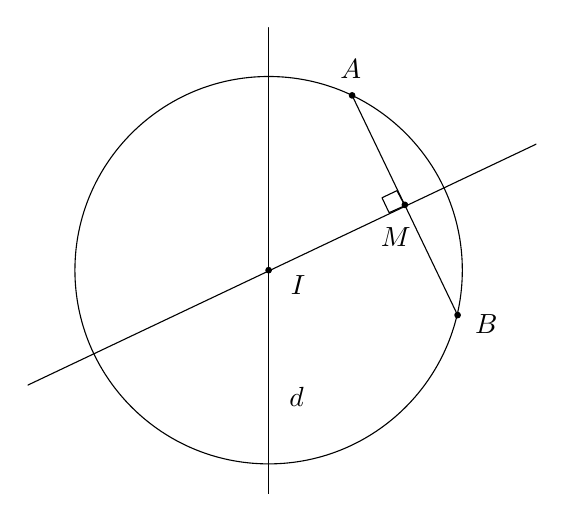
\begin{tikzpicture}[line cap=round,line join=round,>=stealth,x=1.0cm,y=1.0cm]
\clip(1.24,-1.) rectangle (7.7,4.92);
\draw (5.93,2.85) -- (5.74,2.76) -- (5.83,2.57) -- (6.03,2.66) -- cycle;
\draw (4.3,1.84) circle (2.46cm);
\draw (5.36,4.06)-- (6.7,1.27);
\draw [domain=1.24:7.7] plot(\x,{(-0.36--0.82*\x)/1.73});
\draw (4.3,-1.) -- (4.3,4.92);
\draw (5.6,4.4) node[left] {$A$};
\draw (6.8,1.4) node[anchor=north west] {$B$};
\draw (5.6,2.5) node[anchor=north west] {$M$};
\draw (4.44,0.48) node[anchor=north west] {$d$};
\draw (4.46,1.9) node[anchor=north west] {$I$};
\draw [fill=black] (4.3,1.84) circle (1.0pt);
\draw [fill=black] (5.36,4.06) circle (1.0pt);
\draw [fill=black] (6.7,1.27) circle (1.0pt);
\draw [fill=black] (6.03,2.67) circle (1.0pt);
\end{tikzpicture}
}
}
\end{ex}
\TL
\begin{ex}%[0H9H3-2]%[Dự án đề kiểm tra Toán 10 HKII NH23-24-Đỗ Chí Tâm]%[THPT Đặng Huy Trứ- Huế]
Trong mặt phẳng với hệ trục tọa độ $Oxy$, cho hai điểm $A(2;-3), B(4;1)$. Gọi $\Delta$ là đường thẳng trung trực của đoạn $AB$. Viết phương trình tham số của đường thẳng $\Delta$.
\loigiai{
Trung điểm của $AB$ là $I(3;-1)$.\\
Vectơ pháp tuyến của đường thẳng $\Delta$ là $\vec{n_{\Delta}}=\vec{AB}=(2;4)$.\\
Đường thẳng $\Delta$ đi qua trung điểm $I(3;-1)$ của $AB$ và có vectơ chỉ phương $\vec{u_{\Delta}}=(4;-2)$, có phương trình là $\heva{&x=3+4t\\&y=-1-2t}\quad t\in\mathbb{R}$.

}
\end{ex}

\begin{ex}%[0H9V4-5]%[Dự án đề kiểm tra Toán 10 HKII NH23-24- Trung Anh]%[THPT Việt Đức - Hà Nội]
Trong mặt phẳng với hệ trục tọa độ $Oxy$, cho đường tròn $(C): x^2+y^2+4x-2y-20=0$ và đường thẳng $\triangle: 3x+4y-m=0$. Tìm giá trị dương của tham số $m$ để đường thẳng $\triangle$ cắt đường tròn $(C)$ theo một dây dung có độ dài bằng $6$.
\loigiai{
\begin{center}
\begin{tikzpicture}[declare function={r=2.5;ga=40;},>=stealth,font=\scriptsize,scale=0.8]
%\path (0:0) coordinate (I)
%(ga:r) coordinate (A)
%(130:r) coordinate (B)
\coordinate (I) at (0,0);
\coordinate (A) at (ga:r);
\coordinate (B) at (130:r);
\coordinate (J) at ($(A)!1/2!(B)$);
\draw (I) circle (r)  ;
\draw (I)--(A)--(B)--(I)--(J);
\foreach \x/\g in{A/90,B/90,J/90,I/-90}
\fill[black](\x) circle (2pt)
($(\x)+(\g:5mm)$) node{\small $\x$};
\end{tikzpicture}
\end{center}
Đường tròn $(C)$ có tâm $I(-2;1)$ và bán kính $R=\sqrt{(-2)^2+1^2+20}=5$.\\
Giả sử $\triangle$ cắt $(C)$ tại hai điểm $A$ và $B$. Gọi $J$ là trung điểm của $AB$.\\
Khi đó $\heva{&IJ\perp AB\\&JB=\dfrac{1}{2}AB=3.}$\\
Xét tam giác $IJB$ vuông tại $J$ có \[IJ=\sqrt{IB^2-JB^2}=4.\]
Hay $\mathrm{d}(I; \triangle)=4$. Tương đương
\begin{align*}
&\dfrac{|(-2)\cdot3+4\cdot1-m|}{\sqrt{3^+4^2}}=4\\
\Leftrightarrow&\, |m+2|=4\cdot5=20\\
\Leftrightarrow&\, \hoac{&m+2=20\\&m+2=-20}\Leftrightarrow\hoac{&m=18\\&m=-22\,(\text{không thỏa mãn}).}
\end{align*}
Vậy $m=18$.
}
\end{ex}

\begin{ex}%[Phan Quốc Trí]%[0D0C2-7]
Gọi $X$ là tập hợp các số tự nhiên chẵn có $4$ chữ số khác nhau được lập từ các chữ	số $0$; $2$; $3$; $4$; $5$; $6$; $7$. Chọn ngẫu nhiên một số thuộc tập $X$. Tính xác suất để số được chọn chia hết cho $4$ (làm tròn đến hàng phần nghìn).
% \shortans{$0{,}495$}
\loigiai
{
Gọi $\overline{abcd}$ là số tự nhiên chẵn có $4$ chữ số khác nhau được lập từ các chữ số $0$; $2$; $3$; $4$; $5$; $6$; $7$.\\ Các khả năng xảy ra là
\begin{itemize}
\item $d=0$: $a$ có $6$ cách chọn, $b$ có $5$ cách chọn, $c$ có $4$ cách chọn. Có $6\cdot 5\cdot 4=120$ số như vậy.
\item $d\in \{2;4;6\}\Rightarrow d$ có $3$ cách chọn, $a$ có $5$ cách chọn, $b$ có $5$ cách chọn, $c$ có $4$ cách chọn. Có $3\cdot 5\cdot 5\cdot 4=300$ số như vậy.
\end{itemize}
Số phần tử của không gian mẫu là $n(\Omega)=120+300=420$.\\
Gọi $A$ là biến cố \lq\lq Số được chọn chia hết cho $4$\rq\rq.\\
Các khả năng xảy ra là
\begin{itemize}
\item $\overline{cd}\in \{04;20;40;60\}$, $\overline{cd}$ có $4$ cách chọn, $a$ có $5$ cách chọn, $b$ có $4$ cách chọn. Có $4\cdot 5\cdot 4=80$ số như vậy.
\item $\overline{cd}\in \{24;32;36;52;56;64;72;76\}$, $\overline{cd}$ có $8$ cách chọn, $a$ có $4$ cách chọn, $b$ có $4$ cách chọn.\\ Có $8\cdot 4\cdot 4=128$ số như vậy.
\end{itemize}
Số phần tử của biến cố $A$ là $n(A)=80+128=208$.\\
Xác suất cần tìm là $\mathrm{P}(A)=\dfrac{n(A)}{n(\Omega)}=\dfrac{208}{420}=\dfrac{52}{105} \approx 0{,}495$.
}
\end{ex}
\Closesolutionfile{ans}
\Closesolutionfile{ansbook}
>>>>>>> 33890a9ce1cfbd3079ed36a93e836cf3ef1fde30
